\documentclass[a4paper,12pt]{article} 
% 使用ctex包支持中文
\usepackage{ctex}

\usepackage{tikz}
\usetikzlibrary{karnaugh}

\usepackage{lmodern}
\usepackage{amsmath}

\usepackage{array} % 可选,用于更好的表格格式控制

\usepackage{microtype}

% 开始文档
\begin{document}
% 创建标题页的内容
\title {数值判别电路}
\author{11223128 梁宇凡}
\date{2024-10-23}
% 生成标题
\maketitle

\section{实验内容}

1. 用门电路设计一个组合逻辑电路,它接收一位8421BCD码$B_3B_2B_1B_0$,仅当 $2<B_3B_2B_1B_0<7$时输出Y才为1

2. 用门电路设计一个组合逻辑电路,它接收4位2进制数$B_3B_2B_1B_0$,仅当 $2<B_3B_2B_1B_0<7$时输出Y才为1

\section{实验方案设计}
\subsection{列出真值表}
使用网站https://www.tablesgenerator.com/ ,先在word中输入表格,再整体复制到网站

\begin{table}[h]
    \begin{minipage}{0.48\textwidth}
        \centering
        \textbf{实验一:一位BCD码}
        \begin{tabular}{|l|l|l|l|l|}
            \hline
            \textbf{B0} & \textbf{B1} & \textbf{B2} & \textbf{B3} & \textbf{Y} \\ \hline
            0           & 0           & 0           & 0           & 0          \\ \hline
            0           & 0           & 0           & 1           & 0          \\ \hline
            0           & 0           & 1           & 0           & 0          \\ \hline
            0           & 0           & 1           & 1           & 1          \\ \hline
            0           & 1           & 0           & 0           & 1          \\ \hline
            0           & 1           & 0           & 1           & 1          \\ \hline
            0           & 1           & 1           & 0           & 1          \\ \hline
            0           & 1           & 1           & 1           & 0          \\ \hline
            1           & 0           & 0           & 0           & 0          \\ \hline
            1           & 0           & 0           & 1           & 0          \\ \hline
        \end{tabular}
    \end{minipage}
    \hfill
    \begin{minipage}{0.48\textwidth}
        \centering
        \textbf{实验二:4位二进制数}
        
        \begin{tabular}{|l|l|l|l|l|}
            \hline
            \textbf{B0} & \textbf{B1} & \textbf{B2} & \textbf{B3} & \textbf{Y} \\ \hline
            0           & 0           & 0           & 0           & 0          \\ \hline
            0           & 0           & 0           & 1           & 0          \\ \hline
            0           & 0           & 1           & 0           & 0          \\ \hline
            0           & 0           & 1           & 1           & 1          \\ \hline
            0           & 1           & 0           & 0           & 1          \\ \hline
            0           & 1           & 0           & 1           & 1          \\ \hline
            0           & 1           & 1           & 0           & 1          \\ \hline
            0           & 1           & 1           & 1           & 0          \\ \hline
            1           & 0           & 0           & 0           & 0          \\ \hline
            1           & 0           & 0           & 1           & 0          \\ \hline
            1           & 0           & 1           & 0           & 0          \\ \hline
            1           & 0           & 1           & 1           & 0          \\ \hline
            1           & 1           & 0           & 0           & 0          \\ \hline
            1           & 1           & 0           & 1           & 0          \\ \hline
            1           & 1           & 1           & 0           & 0          \\ \hline
            1           & 1           & 1           & 1           & 0          \\ \hline
        \end{tabular}
    \end{minipage}
\end{table}

\newpage

\subsection{绘制卡诺图}
\textbf{实验一:一位BCD码}

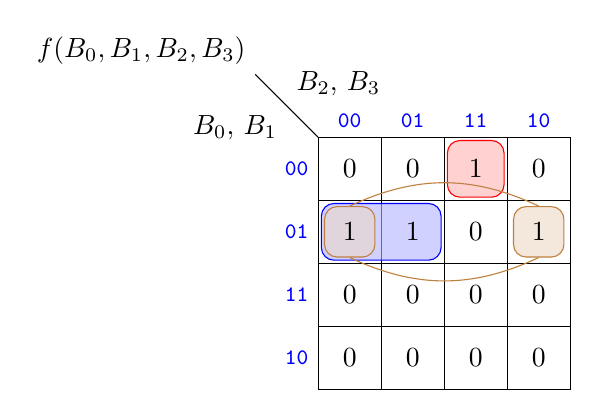
\begin{tikzpicture}[karnaugh, American style, 
    grp/.style n args={3}{#1,fill=#1!30,
    minimum width=#2\kmunitlength,
    minimum height=#3\kmunitlength,
    rounded corners=0.2\kmunitlength,
    fill opacity=0.6,
    rectangle,draw}]
    \karnaughmap{4}{$f(B_0,B_1,B_2,B_3)$}{{$B_0$}{$B_2$}{$B_1$}{$B_3$}}%
       {0011 0110 0000 0000}%
       {
          \node[grp={blue}{1.9}{0.9}](n000) at (1.0,2.5) {};
          \node[grp={red}{0.9}{0.9}](n001) at (2.5,3.5) {};
          \node[grp={brown}{0.8}{0.8}](n002) at (3.5,2.5) {};
          \node[grp={brown}{0.8}{0.8}](n003) at (0.5,2.5) {};
          \draw[brown] (n002.north) to [bend right=25] (n003.north)
                       (n002.south) to [bend left=25] (n003.south);
       }
\end{tikzpicture}



\iffalse

          \node[grp={blue}{1.9}{0.9}](n000) at (1.0,2.5) {};
          \node[grp={red}{0.9}{0.9}](n001) at (2.5,3.5) {};
          \node[grp={brown}{0.9}{0.9}](n002) at (3.5,2.5) {};



            \node[grp={blue}{1.9}{1.9}](n000) at (1.0,2.0) {};
            \node[grp={red}{0.9}{0.9}](n001) at (2.5,3.5) {};
            \node[grp={brown}{0.8}{1.8}](n002) at (3.5,2.0) {};
            \node[grp={brown}{0.8}{1.8}](n003) at (0.5,2.0) {};
            \draw[brown] (n002.north) to [bend right=25] (n003.north)
                         (n002.south) to [bend left=25] (n003.south);
          
          \node[grp={blue}{1.9}{1.9}](n000) at (1.0,2.0) {};
          \node[grp={red}{0.9}{0.9}](n001) at (2.5,3.5) {};
          \node[grp={red}{0.9}{0.9}](n002) at (2.5,0.5) {};
          \draw[red] (n001.west) to [bend right=25] (n002.west)
                     (n001.east) to [bend left=25] (n002.east);
          \node[grp={green}{0.8}{1.8}](n003) at (3.5,2.0) {};
          \node[grp={green}{0.8}{1.8}](n004) at (0.5,2.0) {};
          \draw[green] (n003.north) to [bend right=25] (n004.north)
                       (n003.south) to [bend left=25] (n004.south);
\fi

\subsection{逻辑化简}
实验一:一位BCD码

由卡诺图得,
\begin{align}
     Y&=\bar{B_1}B_2B_3+B_1\bar{B_2}+B_1\bar{B_3} \\
      &=\overline{\overline{\bar{B_1}B_2B_3+B_1\bar{B_2}+B_1\bar{B_3}}}\\
      &=\overline{B_1\overline{B_2B_3}\cdot\overline{\bar{B_1}B_2B_3}}
\end{align}

实验二:4位二进制数

由卡诺图得,
\begin{align}
     Y&=\bar{B_0}B_1\bar{B_2}+\bar{B_0}\bar{B_1}B_2B_3+\bar{B_0}B_1\bar{B_3}\\
      &=\overline{\overline{\bar{B_0}B_1\overline{B_2B_3}}\cdot\overline{\bar{B_0}\bar{B_1}B_2B_3}}
\end{align}

\subsection{逻辑电路图}
\textbf{实验一:一位BCD码  (非门用与非门实现)}
\iffalse
\begin{figure}[h]
   \centering
   \includegraphics[width=0.8\textwidth]{./figures/lab2-1.png}
   \caption{实验一逻辑电路图}
\end{figure}

\textbf{实验二:4位二进制数}
\begin{figure}[h]
   \centering
   \includegraphics[width=0.8\textwidth]{./figures/lab2-2.png}
   \caption{实验二逻辑电路图}
\end{figure}

\fi
\subsection{测试方案}
4个输入信号,用实验箱上的逻辑电平开关实现,1个输出端连接到实验箱上的LED,按照真值表的要求,拨动逻辑电平开关改变输入信号值,遍历16种输入组合,并观察输出信号值,输出 LED亮则输出为1,灭则输出为 0,将测试结果填入下表中。


\begin{table}[h]
   \begin{minipage}{0.48\textwidth}
       \centering
       \textbf{实验一:一位BCD码}
       \begin{tabular}{|l|l|l|l|l|}
           \hline
           \textbf{B0} & \textbf{B1} & \textbf{B2} & \textbf{B3} & \textbf{测试结果} \\ \hline
           0           & 0           & 0           & 0           & 0          \\ \hline
           0           & 0           & 0           & 1           & 0          \\ \hline
           0           & 0           & 1           & 0           & 0          \\ \hline
           0           & 0           & 1           & 1           & 1          \\ \hline
           0           & 1           & 0           & 0           & 1          \\ \hline
           0           & 1           & 0           & 1           & 1          \\ \hline
           0           & 1           & 1           & 0           & 1          \\ \hline
           0           & 1           & 1           & 1           & 0          \\ \hline
           1           & 0           & 0           & 0           & 0          \\ \hline
           1           & 0           & 0           & 1           & 0          \\ \hline
       \end{tabular}
   \end{minipage}
   \hfill
   \begin{minipage}{0.48\textwidth}
       \centering
       \textbf{实验二:4位二进制数}
       
       \begin{tabular}{|l|l|l|l|l|}
           \hline
           \textbf{B0} & \textbf{B1} & \textbf{B2} & \textbf{B3} & \textbf{测试结果} \\ \hline
           0           & 0           & 0           & 0           & 0          \\ \hline
           0           & 0           & 0           & 1           & 0          \\ \hline
           0           & 0           & 1           & 0           & 0          \\ \hline
           0           & 0           & 1           & 1           & 1          \\ \hline
           0           & 1           & 0           & 0           & 1          \\ \hline
           0           & 1           & 0           & 1           & 1          \\ \hline
           0           & 1           & 1           & 0           & 1          \\ \hline
           0           & 1           & 1           & 1           & 0          \\ \hline
           1           & 0           & 0           & 0           & 0          \\ \hline
           1           & 0           & 0           & 1           & 0          \\ \hline
           1           & 0           & 1           & 0           & 0          \\ \hline
           1           & 0           & 1           & 1           & 0          \\ \hline
           1           & 1           & 0           & 0           & 0          \\ \hline
           1           & 1           & 0           & 1           & 0          \\ \hline
           1           & 1           & 1           & 0           & 0          \\ \hline
           1           & 1           & 1           & 1           & 0          \\ \hline
       \end{tabular}
   \end{minipage}
\end{table}

\end{document}